%--------Métricas
%--------Daniel Quinteros Céspedes
%--------23-09-2014

\chapter{Análisis de resultados obtenidos}
\label{cap:analisis}

Un vez completado el proceso de evaluación (Cap.~\ref{cap:eval}) el siguiente paso corresponde al análisis, el cual es tema principal de este capítulo. El análisis comparativo se realizará en tres etapas. En primer lugar se analizarán todos los resultados de manera general. En segundo lugar se realizarán las comparativas entre un algoritmo y otro, finalmente se analizará el comportamiento con la métricas propuesta. 


\section{Análisis generales}
\label{analisis:compgeneral}

En las comparaciones generales se revisarán e ilustrarán los aspectos cuantitativos de los resultados, esto es cantidad de resultados obtenidos y apreciaciones sobre los tiempos para el cálculo de todas las matrices resultados. Por otra parte se analizará las dimensiones del set de datos utilizados y las transformaciones realizadas sobre el mismo para su adecuación al problema analizado. 

\subsection{Dimensión del set de datos y resultados obtenidos}

El set de datos INRIA consta de un total de 6121 imágenes divididas en grupos de, entrenamiento (positivo, con peatón y negativo, sin peatón),  pruebas (positivo y negativo) y ejemplos normalizados de entrenamiento y pruebas (solo positivos) como se indica en la tabla~\ref{tab:inria}.

 \begin{table}[H]
 \centering
  \caption{\em Cantidad de imaǵenes en el set de datos INRIA según tipo.}  
  \label{tab:inria}
\begin{tabular}{lcc|c|c|}
\cline{2-5}
\multicolumn{1}{l|}{}               & \multicolumn{1}{c|}{Postivo} & Negativo              & Normalizado (Solo positivas) & Totales \\ \hline
\multicolumn{1}{|l|}{Entrenamiento} & \multicolumn{1}{c|}{614}     & 1218                  & 2416                         & 4248    \\ \hline
\multicolumn{1}{|l|}{Pruebas}       & \multicolumn{1}{c|}{288}     & 453                   & 1132                         & 1873    \\ \hline
                                    & \multicolumn{1}{l}{}         & \multicolumn{1}{l|}{} & \multicolumn{1}{r|}{Total}   & 6121    \\ \cline{4-5} 
\end{tabular}
\end{table}

Para todas las imágenes positivas sin normalizar, tanto de entrenamiento como de pruebas, existen anotaciones para todos lo peatones. Un total de 902 anotaciones (ver ejemplo en fig.~\ref{fig:ejanotacion}) que ayudaron en el proceso para la normalización a diferentes escalas. En particular se extrajo una versión escalada del set original tanto para entrenamiento y pruebas, además se utilizaron 9120 ejemplos negativos extraídos de forma aleatoria de las imágenes negativas de entrenamiento. En la tabla~\ref{tab:useddataset} se puede observar la cantidad de imágenes obtenidas según tamaño de ventana de clasificación.

\begin{table}[h]
\caption{\em Cantidad de imaǵenes en el set de datos utilizado según ventana de clasificación.}  
  \label{tab:useddataset}
  \resizebox{15cm}{!} {
\begin{tabular}{lcc|c|c|}
\hline
\multicolumn{1}{|l|}{Ventana}   & \multicolumn{1}{c|}{Entrenamiento Positivos} & Entrenamiento Negativos & Pruebas (Solo positivos)   & Totales                    \\ \hline
\multicolumn{1}{|l|}{32x64px}   & \multicolumn{1}{c|}{614}                     & -                       & 589                        & 1203                       \\ \hline
\multicolumn{1}{|l|}{64x128px}  & \multicolumn{1}{c|}{614}                     & 9120                    & 589                        & 10323                      \\ \hline
\multicolumn{1}{|l|}{128x256px} & \multicolumn{1}{c|}{614}                     & -                       & 589                        & 1203                       \\ \hline
\multicolumn{1}{|l|}{256x512px} & \multicolumn{1}{c|}{614}                     & -                       & 589                        & 1203                       \\ \hline
                                & \multicolumn{1}{l}{}                         & \multicolumn{1}{l|}{}   & \multicolumn{1}{r|}{Total} & \multicolumn{1}{l|}{13932} \\ \cline{4-5} 
\end{tabular}}
\end{table}
 
 
Dado que la transformación de tamaño de los negativos para el entrenamiento se realiza de forma dinámica, se tomó ejemplos solo para el tamaño de clasificación sugerido por \cite{dalal2006}, 64x128px. Esto permite que todos los entrenamientos se realicen con los mismos negativos. En el caso de los positivos el parámetro invariante corresponde a la vecindad \ie se consideró una vecindad fija respecto del peatón (una razón vecindad/peatón) en su imagen original y luego se escaló dicha vecindad a los tamaños muchas veces mencionados.
Para cada imágenes de prueba (598) se obtuvo una matriz resultado de la detección. Como la detección se realizó por dos combinaciones de descriptor/clasificador se obtuvo un total del 4712 matrices. 


\subsection{Tiempos para la clasificación}

Los tiempos de la clasificación no fueron tomados de forma precisa por lo que solo se presentarán apreciaciones. Es importante mencionar el aspecto temporal del proceso aún cuando no se tengan las medidas precisas. No se esperaba que el aspecto temporal fuera algo relevante a la hora de realizar la evaluación. Sin embargo, el tiempo que demoró completar el proceso fue mayor que los esperado. Lo anterior sucede porque la cantidad de clasificaciones crece de forma importante en la medida que aumenta la ventana de clasificación. Esto se debe a que si crece la ventana, pero queremos mantener fija la razón de vecindad/peatón y el tamaño de la ventana tiene una relación directamente proporcional con el tamaño del peatón, entonces el tamaño de la vecindad debe aumentar en esa misma medida. En el gráfico de la figura~\ref{fig:grow} se puede observar el crecimiento de la cantidad de detecciones necesarias (para mantener la razón vecindad/peatón) según el tamaño de la ventana. 

\begin{figure}[H]
  \centering
  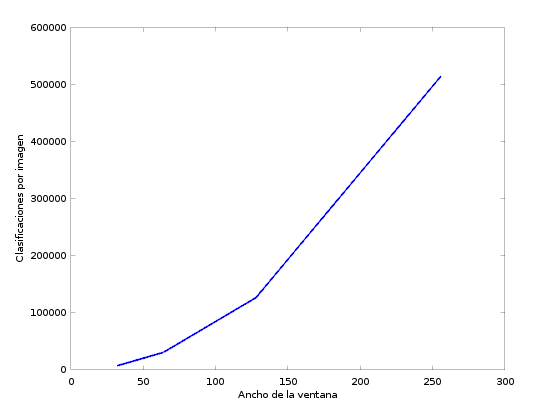
\includegraphics[scale=.6]{images/clasgrow}
  \caption{\em Crecimiento de la cantidad de clasificaciones necesarias por imagen de acuerdo al ancho de la ventana de clasificación..}  
  \label{fig:grow}
\end{figure}

Evidentemente realizar cada vez cantidad de clasificaciones requiere cada vez más tiempo. De esta manera el tiempo aproximado en realizar la tarea de detección para todo el set de datos con una ventana de clasificación de 32x64px toma una hora. Esto es utilizando una configuración de hardware como la descrita en al Anexo~\ref{cap:manual}. Por lo que para realizar la clasificación para las ventana más grandes (128x256px y 256x512px) se utilizó un cluster con 32 núcleos al cual le llevó aproximadamente una semana en realizar todas las clasificaciones para todas las imágenes en ambas configuraciones de detector/clasificador. Se realizaron un total de 800.078.752 clasificaciones. Esta cantidad de clasificaciones fueron realizadas en paralelo para reducir su tiempo de cómputo utilizando OpenMP.

 
\section{Comparación por algoritmo}
\label{analisis:compalgoritmo}

En la comparación por algoritmo se analizará la métrica seleccionada (Promedio ponderado de las diferencias) enfocado en la comparación entre algoritmos, para esto se revisaran la comparaciones a nivel gráfico y estadístico descriptivo.%**estadístico inferencial. 

La primera sección de la comparación por algoritmos será basada en la inspección visual de los gráficos y apoyada por el cálculo de PPD, la cantidad de resultados obtenido no permite realizar gráficos de todos ellos y mucho menos exponerlos en esta sección por lo que se pondrán encontrar más ejemplos en el Anexo~\ref{cap:gre}. 

\subsection{Comparación gráfica}

En la figura~\ref{fig:prueba1} hay dos gráficos que se obtuvieron luego de la etapa de detección, estos gráficos corresponden detecciones sin normalizar. Ambos gráficos representan la detección de la misma imagen. El gráfico detección utilizando HOG/Adaboost es mucho más ``aspero'' que el de la combinación HOG/SVM lineal. Para el post procesamiento es deseable una mayor suavidad ya que en general se utilizan algoritmo para la búsqueda de máximos locales lo que pueden quedar detenidos en máximo local menor, por lo que el descriptor/clasificador de elección sería HOG/SVM. Se puede observar una elevación en el centro de ambos gráficos lo que representa la detección correcta del peatón. Sin embargo hay una cantidad apreciable de ruido en ambos gráficos hacia la parte superior. 

\begin{figure}[H]
  \centering
  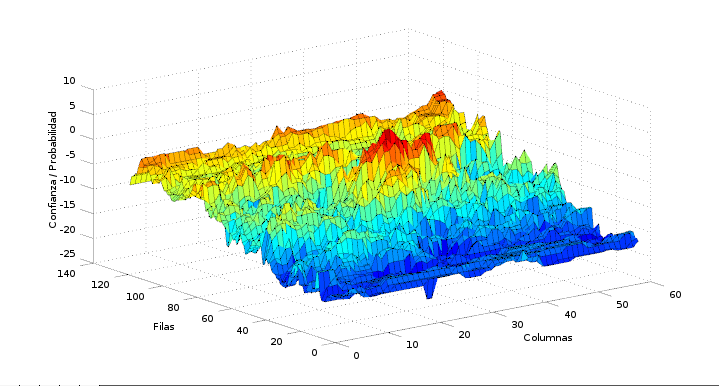
\includegraphics[scale=.27]{images/raw/boost/prueba}
  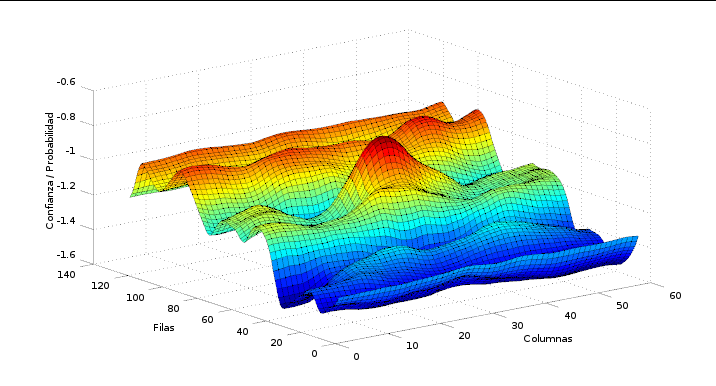
\includegraphics[scale=.27]{images/raw/svm/prueba}
  \caption{\em Resultados ``crudos'' obtenidos de la detección sobre una sola imagen utilizando una ventana deslizante de 32x64px. A la izquierda, obtenido con la combinación descriptor/clasificador HOG/Adaboost. A la derecha, obtenido con la combinación descriptor/clasificador HOG/SVM lineal.}  
  \label{fig:prueba1}
\end{figure}

Luego del proceso de normalización utilizando el método de \cite{Platt1999} se obtienen gráficos como el de la figura~\ref{fig:prueba2}. Los gráficos corresponde a la detección de la misma imagen que los de la figura~\ref{fig:prueba1}. El primer elemento a destacar es la gran reducción de ruido que se produce. El gráfico de HOG/Adaboost presenta ahora un diferencia mucho más notoria que en la comparación con el gráfico de HOG/SVM. La combinación HOG/Adaboost tiene un resultado que se observa dicotómico \ie para un punto evaluado hay 
o no una persona, sin matices. La combinación HOG/SVM parece detectar una mayor cantidad de ruido que la combinación HOG/Adaboost. Considerando que se planteó que la respuesta ideal del clasificador debería ser similar a un impulso el gráfico de HOG/Adaboost parece representar mayor sensibilidad dado el tipo de respuesta. Sin embargo los errores también serán más ``castigados'' por lo que esta apreciación no es la correcta.

\begin{figure}[H]
  \centering
  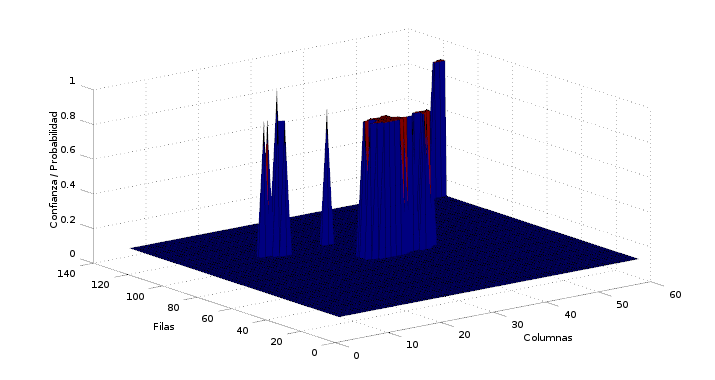
\includegraphics[scale=.25]{images/sig/boost/prueba}
  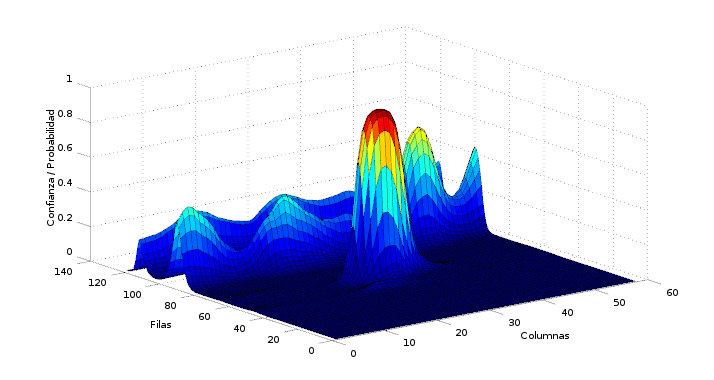
\includegraphics[scale=.25]{images/sig/svm/prueba}
  \caption{\em  Resultados probabilísticos obtenidos de la detección de una sola imagen utilizando una ventana deslizante de 32x64px. A la izquierda, obtenido de la combinación descriptor/clasificador HOG/Adaboost. A la derecha, obtenido con la combinación descriptor/clasificador HOG/SVM lineal.}  
  \label{fig:prueba2}
\end{figure}

Al realizar la evaluación de estos gráficos con la métrica de sensibilidad PPD se obtiene los resultados que se exponen en la tabla~\ref{tab:resp2}. Se puede observar que el valor de sensibilidad es mejor en el caso de HOG/SVM que en el caso de HOG/Adaboost.

\begin{table}[H]
\centering
 \caption{\em  Valores de sensibilidad espacial según PPD para los gráficos de la figura~\ref{fig:prueba2}. Menos es mejor}  
  \label{tab:resp2}
\begin{tabular}{l|l|}
\cline{2-2}
                                      & PPD     \\ \hline
\multicolumn{1}{|l|}{HOG/Adaboost}    & 5.0898 \\ \hline
\multicolumn{1}{|l|}{HOG/SVM lineal} &  1.2484 \\ \hline
\end{tabular}
\end{table}

Con el objetivo de tener una visión general de la detección realizada por cada clasificador los gráficos de las figuras~\ref{fig:mean1} y~\ref{fig:mean2} representan el promedio de los resultados obtenidos para cada combinación descriptor/clasificador.
En el primer caso (\ref{fig:mean1}) se utilizó una ventana deslizante de 64x128px. Los resultados de ambas combinaciones del descriptor clasificador muestran gran similitud, muy contrario a lo visto en la evaluación de una única imagen. Aun luego de todo el proceso el gráfico obtenido con HOG/SMV conserva una mayor suavidad que el obtenido con HOG/Adaboost. 

\begin{figure}[H]
  \centering
  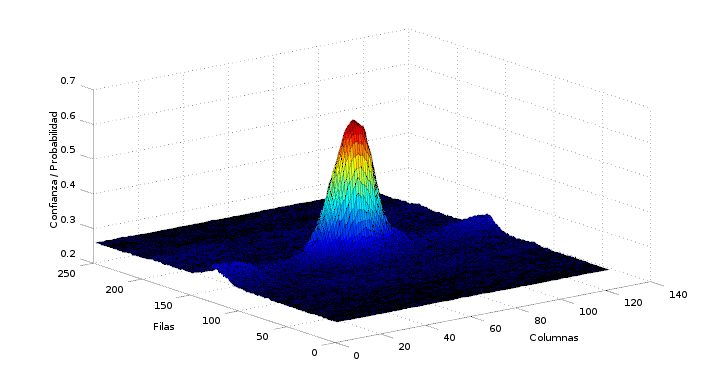
\includegraphics[scale=.25]{images/mean/boost/64}
  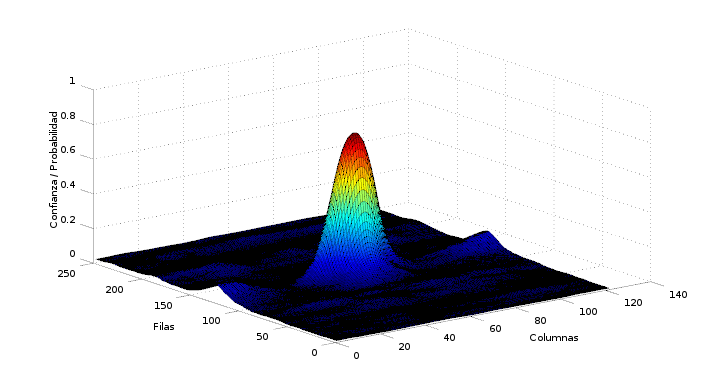
\includegraphics[scale=.25]{images/mean/svm/64}
  \caption{\em  Resultados promedio de la detección de todas las imágenes del set de datos utilizando una ventana deslizante de 64x128px. A la izquierda, obtenido de la combinación descriptor/clasificador HOG/Adaboost. A la derecha, obtenido con la combinación descriptor/clasificador HOG/SVM lineal.}  
  \label{fig:mean1}
\end{figure}

En la figura~\ref{fig:mean2} se utilizó una ventana de detección más grande que la anterior (128x256px) el resultado en forma gráfica no tiene mayores diferencias o similitudes que en el caso de la figura anterior (fig.~\ref{fig:mean1}).
En general en los resultados de los gráficos promedio se puede observar una elevación mayor en el centro de cada gráfico que se puede traducir como la detección correcta promedio. Por otra parte a los costados de la elevación principal se observan elevaciones menores. Las elevaciones se encuentran en el eje horizontal de la detección y por tanto de la imagen, por lo que son interpretadas como detecciones a los costados del peatón. Esta es una situación razonable si se piensa que muchos peatones en el conjunto de datos se encuentran lado a lado con otros, por lo que forman parte de su vecindad cercana. Entonces estas elevaciones corresponden a la detección de dichos peatones. 

\begin{figure}[H]
  \centering
  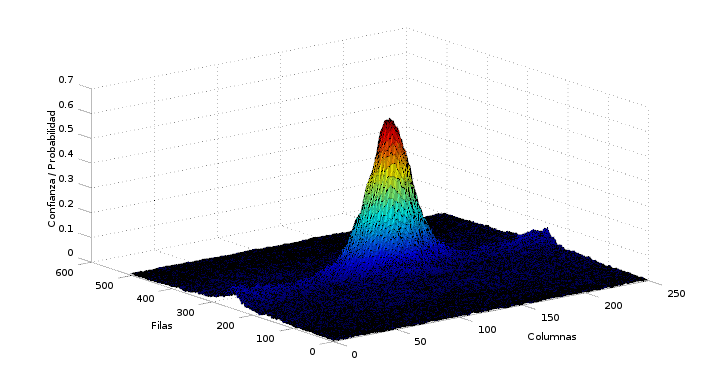
\includegraphics[scale=.25]{images/mean/boost/128}
  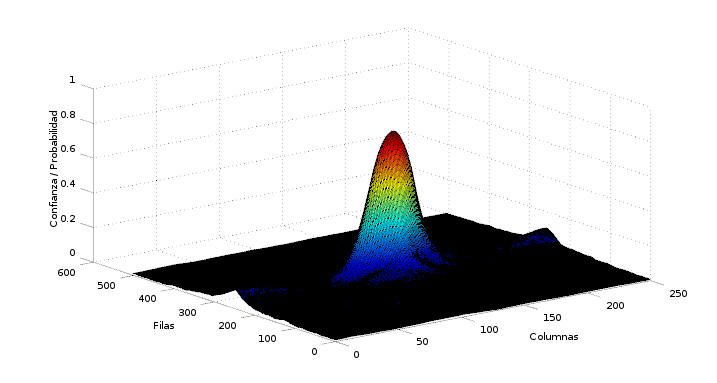
\includegraphics[scale=.25]{images/mean/svm/128}
  \caption{\em  Resultados promedio de la detección de todas las imágenes del set de datos utilizando una ventana deslizante de 128x256px. A la izquierda, obtenido de la combinación descriptor/clasificador HOG/Adaboost. A la derecha, obtenido con la combinación descriptor/clasificador HOG/SVM lineal.}  
  \label{fig:mean2}
\end{figure}

En total detecciones en promedio realizadas por cada clasificador tienen un valor de sensibilidad promedio que se puede observar en la tabla~\ref{tab:prom1}, en la cual se observamos que el valor de sensibilidad espacial promedio de HOG/SVM es mejor que el valor de HOG/Adaboost.

\begin{table}[h]
\centering
\caption{\em  Valores promedio de sensibilidad espacial PPD por clasificador. Menos es mejor}  
\label{tab:prom1}
\begin{tabular}{l|l|}
\cline{2-2}
                                      & PPD Promedio \\ \hline
\multicolumn{1}{|l|}{HOG/Adaboost}    & 11.065     \\ \hline
\multicolumn{1}{|l|}{HOG/SVM lineal}  & 3.489      \\ \hline
\end{tabular}
\end{table}

La comparación de los gráficos entrega información general respecto la sensibilidad espacial y del funcionamiento de los detectores de personas. Los datos que entregan los gráficos al análisis visual son en general cualitativos por lo que cuando las similitudes son altas la diferenciación es compleja. Para ilustrar el plano general de los resultados obtenidos se utilizará una tabla resumen (\ref{tab:resumengrafico}) de diferencias y semejanzas a nivel de la comparación de todos los gráficos presentados e información extra obtenida de los gráfico en el Anexo~\ref{cap:gre}.

\begin{table}[h]
\centering
\caption{\em Resumen análisis visual de los gráficos expuestos.}  
\label{tab:resumengrafico}
\resizebox{15cm}{!} {
\begin{tabular}{l|l|l|}
\cline{2-3}
\rowcolor[HTML]{C0C0C0} 
\cellcolor[HTML]{FFFFFF}                                                                                                            & \multicolumn{1}{c|}{\cellcolor[HTML]{C0C0C0}Similitudes}                                                                                                                                                  & \multicolumn{1}{c|}{\cellcolor[HTML]{C0C0C0}Diferencias}                                                                                                                                                                                                               \\ \hline
\multicolumn{1}{|l|}{\cellcolor[HTML]{C0C0C0}\begin{tabular}[c]{@{}l@{}}Resultados ``crudos''\\ para una sola imagen\end{tabular}}    & \begin{tabular}[c]{@{}l@{}}- La elevación central es signo \\ de la correcta detección del peatón \\ en el centro de la imagen.\\ - La cantidad y tipo de ruido\\  detectado es muy similar.\end{tabular} & \begin{tabular}[c]{@{}l@{}}- El gráfico de HOG/SVM es más \\ suave que el de HOG/Adaboost.\end{tabular}                                                                                                                                                                \\ \hline

\multicolumn{1}{|l|}{\cellcolor[HTML]{C0C0C0}\begin{tabular}[c]{@{}l@{}}Resultados normalizados\\ para una sola imagen\end{tabular}} & \cellcolor[HTML]{EFEFEF} - En ambos casos se refuerza la detección central.                                                                                                                                                        & \cellcolor[HTML]{EFEFEF}\begin{tabular}[c]{@{}l@{}}-  Combinación HOG/Adaboost tiene una\\  respuesta abrupta en comparación a la \\ de HOG/SVM.\\ - HOG/SVM presenta una mayor cantidad\\ de clasificaciones con ruido, pero de menor \\ intesidad que el ruido en HOG/Adaboost.\end{tabular} \\ \hline
\multicolumn{1}{|l|}{\cellcolor[HTML]{C0C0C0}Matriz promedio}                                                                       & \begin{tabular}[c]{@{}l@{}}- Los gráficos tiene una figura muy\\  similar con una notoria elevación \\ en el centro.\\ - En ambas combinaciones se \\ observan elevaciones en los laterales.\end{tabular} & \begin{tabular}[c]{@{}l@{}}- EL gráfico de HOG/SVM permanece\\  más suave que el de HOG/Adaboost.\end{tabular}                                                                                                                                                         \\ \hline
\end{tabular}}
\end{table}

Una vez completado el análisis de los gráficos, es importante revisar la comparación de detectores de personas mostrando en detalle los resultados obtenidos con la métrica PPD.

\subsection{Comparación numérica}

Para la caracterización de los valores medidos de sensibilidad espacial se utilizará algunas herramientas básicas de estadística descriptiva. Además se comparará directamente el comportamiento de la métrica entre las diferentes combinaciones de descriptor/clasificador/tamaño de ventana.


\begin{table}[h]
\centering
\caption{\em  Valores PPD promedio y desviación estándar por combinación \\ descriptor/clasificador/tamaño de ventana}  \label{tab:promgeneral}
\resizebox{15cm}{!} {
\begin{tabular}{|l|c|c|c|}
\hline
\rowcolor[HTML]{C0C0C0} 
Detector  -  Tamaño de ventana & PPD promedio & Desviación Estándar & PPD de la matriz promedio       \\ \hline
HOG/SVM - 32x64px              & 1.13632      & 0.68212             & \cellcolor[HTML]{FFFFFF}1.13632 \\ \hline
\rowcolor[HTML]{EFEFEF} 
HOG/Adaboost - 32x64px         & 5.37080      & 0.28299             & 5.37080                         \\ \hline
HOG/SVM - 64x128px             & 1.50811      & 0.87310             & 1.50811                         \\ \hline
\rowcolor[HTML]{EFEFEF} 
HOG/Adaboost - 64x128px        & 19.20734     & 0.26390             & 19.20734                        \\ \hline
HOG/SVM - 128x256px            & 2.62159      & 2.58049             & 2.62159                         \\ \hline
\rowcolor[HTML]{EFEFEF} 
HOG/Adaboost - 128x256px       & 1.47125      & 1.55752             & 1.47125                         \\ \hline
HOG/SVM - 256x512px            & 8.69029      & 10.93515            & 8.69029                         \\ \hline
\rowcolor[HTML]{EFEFEF} 
HOG/Adaboost - 256x512px       & 18.21166     & 19.40539            & 18.21166                        \\ \hline
\end{tabular}}
\end{table}

En la tabla~\ref{tab:promgeneral} se exponen los valores en cada caso de detección. Un valor que llama la atención es de la desviación estándar la cual aumenta su valor de forma considerable en la medida en que aumenta el tamaño de la ventana. Este fenómeno indica que la incertidumbre de la evaluación aumenta conforme aumenta el tamaño de la ventana de clasificación. Este fenómeno se puede observar mejor en las figuras~\ref{fig:gcsvm} y~\ref{fig:gcboost} del anexo~\ref{cap:gre}.

%ES IMPORTANTE REVISAR QUE ESTO ESTE BIEN LOS DE C13 y C13

En general el resultado obtenido por HOG/SVM lineal tiene un valor de sensibilidad espacial mejor que el obtenido por HOG/Adaboost lo que ya se había visto en la tabla~\ref{tab:prom1}. No obstante es importante observar que el valor promedio es menor (menos es mejor) para  cada tamaño de HOG/SVM lineal excepto en 128x256px donde HOG/Adaboost tiene un valor menor. 

\begin{figure}[H]
  \centering
  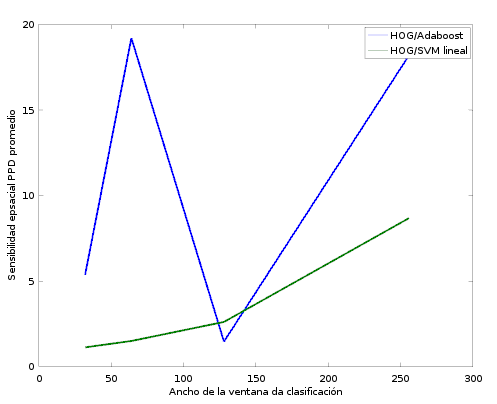
\includegraphics[scale=.5]{images/ssp}
  \caption{\em  En la figura se observa la variación del PPD promedio por combinación descriptor/clasificador}  
  \label{fig:ssp}
\end{figure}

En la figura~\ref{fig:ssp} se expone la variación de PPD promedio por tipo de descriptor/clasificador. En esta figura se puede observar que en el caso de HOG/SVM el valor de PPD aumenta conforme aumenta el tamaño de la ventana. Sin embargo, el valor de PPD para HOG/Adaboost tiene una tendencia que no se encuentra claramente definida. Para determinar una tendencia respecto de HOG/Adaboost se hace necesario obtener más puntos de muestreo intermedios \ie realizar este análisis con una mayor variedad de tamaños de ventanas de clasificación.

Finalmente, producto de la evaluación de la sensibilidad tanto en trabajo realizado por la métrica como por el trabajo realizado en el análisis de gráficos, es posible realizar ahora una elección de un clasificador que ayude a evitar conteos múltiples. Como se insinuó anteriormente y a la vista de los resultados el mejor clasificador resulta ser HOG con SVM lineal ya que tuvo una mejor evaluación. 
A continuación se presentarán brevemente las conclusiones del capítulo.

\section{Conclusiones del capítulo}
\label{analisis:conclusiones}

Producto de la aplicación del trabajo de siete etapas que permitió la evaluación de la sensibilidad espacial de cada uno de los clasificadores mencionado en el capítulo anterior, se generaron resultados sometidos a análisis en este capítulo, siendo este análisis efectuado de tres maneras:
\begin{itemize}
\item Análisis general.
	\subitem 6121 imágenes divididas en conjuntos de entrenamiento, pruebas y ejemplos normalizados de entrenamiento y pruebas, incluyendo imágenes en positivo y negativo.
	\subitem  13932 imágenes en el set de datos considerando las distintas escalas (tamaños de la ventana de clasificación).
	\subitem  4712 matrices de detección.
	\subitem  Más de 800 millones de clasificaciones, realizadas en el espacio aproximado de una semana con la ayuda de un clúster de 32 núcleos, lo que indica la importancia del tiempo a la hora de realizar este tipo de tareas.
\item Comparativa entre algoritmos:
	\subitem Los gráficos de detección producidos por HOG/Adaboost son más ``ásperos'' en comparación a sus similares producidos por HOG/SVM.
	\subitem  La aplicación del método de Platt permite una considerable reducción del ruido presente en los gráficos obtenidos de primera fuente.
	\subitem  Posterior a la aplicación del método, los gráficos de HOG/Adaboost son más tajantes a la hora de determinar si en una determinada región de la imagen se encuentra o no una persona en comparación a HOG/SVM. Pareciera que HOG/Adaboost fuera más sensible espacialmente que HOG/SVM, sin embargo lo tajante que es penaliza de mayor forma los errores de detección, por lo que la apreciación no es del todo correcta.
\item Comportamiento en base a la métrica propuesta: Finalmente, la aplicación de la métrica PPD sobre los gráficos permite determinar que, al contrario de lo pensado inicialmente, la combinación HOG/SVM presenta mejor sensibilidad espacial que HOG/Adaboost, debido a que minimizaría mejor las detecciones múltiples en comparación a HOG/Adaboost para el set de datos de personas INRIA.
\end{itemize}


El análisis comparativo es una herramienta útil para ayudar a la toma de decisiones. La aplicación de esta herramienta en este problema en particular aporta información que ayuda a definir en dos puntos importantes, el post procesamiento y la elección de una combinación descriptor/clasificador para algún problema dado. El análisis visual de gráficos contrastado con la evaluación de la métrica permite tener un amplio espectro que permite caracterizar de buena forma la sensibilidad espacial para una determinada combinación descriptor/clasificador.
Otro punto revisado en este capítulo que resultó importante es la evaluación del tiempo requerido para realizar un estudio de estas características. El cual fue definitivamente superior al esperado.
Finalmente y dados los resultados obtenido HOG/SVM lineal fue escogido como aquel, según indica el objetivo general, que minimizaría la cantidad de múltiples detecciones en el set de datos INRIA, en este caso respecto de HOG/Adaboost. 